\documentclass[UTF8,aspectratio=169,10pt]{ctexbeamer}

\usetheme{Madrid}
\usecolortheme{dolphin}
\setbeamertemplate{navigation symbols}{}
\setbeamertemplate{footline}[frame number]

\usepackage{booktabs}
\usepackage{tabularx}
\usepackage{array}
\usepackage{graphicx}
\usepackage{xcolor}
\usepackage{hyperref}
\usepackage{tikz}
\usetikzlibrary{arrows.meta,positioning}

\definecolor{pgsaBlue}{RGB}{32,74,135}
\definecolor{pgsaGreen}{RGB}{44,129,88}
\definecolor{pgsaOrange}{RGB}{190,104,33}
\definecolor{pgsaRed}{RGB}{168,48,48}
\definecolor{pgsaGray}{RGB}{82,90,99}
\definecolor{pgsaLight}{RGB}{244,247,250}
\definecolor{positive}{RGB}{32,74,135}
\definecolor{negative}{RGB}{190,104,33}
\definecolor{emphasis}{RGB}{44,129,88}
\definecolor{neutral}{RGB}{82,90,99}

\hypersetup{
  colorlinks=true,
  linkcolor=pgsaBlue,
  urlcolor=pgsaBlue
}

\newcommand{\term}[1]{\textcolor{pgsaBlue}{\textbf{#1}}}
\newcommand{\metric}[1]{\textcolor{pgsaGreen}{\textbf{#1}}}
\newcommand{\warn}[1]{\textcolor{pgsaOrange}{\textbf{#1}}}
\newcommand{\risk}[1]{\textcolor{pgsaRed}{\textbf{#1}}}
\newcommand{\pos}[1]{\textcolor{positive}{#1}}
\newcommand{\con}[1]{\textcolor{negative}{#1}}
\newcommand{\HL}[1]{\textcolor{emphasis}{#1}}
\newcommand{\code}[1]{\texttt{#1}}
\newcommand{\source}[1]{\vspace{0.3em}{\footnotesize\textcolor{pgsaGray}{Source: #1}}}
\newcommand{\resultfig}[2][0.70]{\includegraphics[width=\textwidth,height=#1\textheight,keepaspectratio]{#2}}
\newcommand{\takeaway}[1]{\begin{block}{个人复习结论}#1\end{block}}

\setbeamertemplate{blocks}[rounded][shadow=false]
\setbeamercolor{block title}{fg=white,bg=pgsaBlue}
\setbeamercolor{block body}{fg=black,bg=pgsaLight}
\setbeamercolor{alerted text}{fg=pgsaRed}

% Speaker notes are hidden in the normal PDF.
% For a note-enabled review copy, switch this in a local branch or Overleaf:
% \setbeameroption{show notes on second screen=right}
\setbeameroption{hide notes}

\title[PGSA Long-Term Beamer]{并行整体刚度矩阵组装项目长期知识与进展手册}
\subtitle{Parallel Global Stiffness Assembly: background, implementation, benchmark evidence, and roadmap}
\author{Presenter: Jiang Haohua}
\institute{Shanghai Jiao Tong University}
\date{Living deck, first maintained version: 2026-05-15}

\begin{document}

\begin{frame}
  \titlepage
\end{frame}
\note{
这份 deck 不是一次 mentor 汇报稿，而是长期维护的个人知识手册。它的目标是把项目背景、有限元组装基础、C++ 主线实现、benchmark 口径、已有实验结果和下一步路线放在同一个可复习的结构里。后续每次短期汇报结束后，稳定下来的结论应该回流到这份长期 deck。
}

\begin{frame}{如何使用这份长期 deck}
\begin{itemize}
  \item 当成个人项目手册：先读背景，再看实现，再看结果证据。
  \item 当成 mentor 问题索引：遇到 \code{symbolic assembly}、\code{scatter plan}、\code{section/closure} 等概念时，先回到对应章节。
  \item 当成进展账本：短期 beamer 只服务一次汇报，长期 beamer 保存稳定知识和可追溯结论。
  \item 当成复现入口：每张结果图和关键数字都应能追溯到仓库文档、结果包或外部文献。
\end{itemize}
\takeaway{这份材料优先服务“我自己真正理解项目”，不是为了压缩成 7 分钟汇报。}
\end{frame}
\note{
使用顺序建议是：第一次完整通读；以后按问题跳转。比如如果 mentor 问“为什么 symbolic/numeric split 有价值”，就看符号与数值组装章节和 benchmark evidence 章节。如果问“为什么 Apple 和 Intel 的 P/E-core 不能直接比较”，就看平台差异章节。
}

\begin{frame}{全篇结构}
\tableofcontents
\end{frame}

\section{项目定位}

\begin{frame}{项目一句话定位}
\begin{block}{研究对象}
在共享内存多核 CPU 上，研究如何把大量有限元单元刚度矩阵高效、正确地累加到全局稀疏刚度矩阵。
\end{block}
\begin{columns}[T,onlytextwidth]
\begin{column}{0.48\textwidth}
\textbf{不是当前主线}
\begin{itemize}
  \item 继续扩展 GPU 算法。
  \item 做完整商业求解器。
  \item 优化线性方程组求解器。
\end{itemize}
\end{column}
\begin{column}{0.48\textwidth}
\textbf{当前主线}
\begin{itemize}
  \item CPU 并行组装算法对比。
  \item 真实工程网格可复现 benchmark。
  \item 结果、图表、文档和短期汇报可追溯。
\end{itemize}
\end{column}
\end{columns}
\source{README.md; docs/requirements/cpu-parallel-stiffness-assembly-design.md}
\end{frame}
\note{
这个项目的核心不是“有限元所有阶段都优化”，而是聚焦 assembly：从每个 element 的局部刚度矩阵 Ke 出发，把它写回 global stiffness matrix K。求解阶段、边界条件完整处理、非线性材料、MPI 和 GPU 新算法都不是当前主线。
}

\begin{frame}{为什么 assembly 值得单独研究}
\begin{itemize}
  \item 有限元里每个单元都能独立计算局部矩阵，看起来天然并行。
  \item 但多个单元会共享节点和自由度，写回全局矩阵时会写到同一位置。
  \item 因此并行 assembly 的难点不是“算 Ke”，而是\term{如何避免或管理写冲突}。
  \item 真实大网格上，全局矩阵很稀疏，不能用 dense matrix 方式处理。
\end{itemize}
\takeaway{并行 assembly 是“局部计算容易、全局写入困难”的问题。}
\source{docs/requirements/cpu-parallel-stiffness-assembly-design.md; ScienceDirect S0045782524003323}
\end{frame}
\note{
从新手角度理解：每个单元像一小块拼图，Ke 是这块拼图内部自由度之间的刚度关系。把所有拼图放回整体结构时，相邻单元共享边界节点，所以它们会同时贡献到同一个全局矩阵条目。并行时这些共享位置会造成 race condition。
}

\begin{frame}{当前唯一主线目录}
\begin{block}{继续开发入口}
\code{parallel\_global\_stiffness\_assembly/cpu\_parallel\_stiffness\_assembly}
\end{block}
\begin{itemize}
  \item 仓库根 README 已明确：当前项目聚焦 CPU 平台并行整体刚度矩阵组装。
  \item GPU 历史内容保留为 legacy 参考，不是当前默认入口。
  \item 短期 beamer 已在 \code{reports/2026-05-14-mentor-next-steps-beamer/}。
  \item 本长期 beamer 固定放在 \code{reports/project-long-term-beamer/}。
\end{itemize}
\takeaway{后续新增知识、稳定结果和进展复盘，合并到长期 deck；日期目录只承载一次汇报。}
\end{frame}
\note{
这一页是为了防止项目材料散掉。当前仓库里有根 README、docs、results、reports、legacy_gpu 等多类资产。长期 deck 的作用就是把这些资产串成一条学习线。
}

\begin{frame}{项目最终要回答的问题}
\begin{enumerate}
  \item 图着色法在多核 CPU 上是否仍然是合适基线？
  \item 直接累加和 atomic 在真实工程网格上是否可接受？
  \item 线程私有缓冲、COO sort-reduce、row-owner 等路线各自代价是什么？
  \item 规则网格和真实 \code{C3D4} 工程网格上的趋势是否一致？
  \item 工程上后续应该优先保留哪类算法继续优化？
\end{enumerate}
\source{docs/requirements/cpu-parallel-stiffness-assembly-design.md}
\end{frame}
\note{
这些问题来自需求文档。注意它们不是孤立算法题，而是研究平台问题：同一输入、同一 CSR、同一 correctness baseline、同一 benchmark schema 下，比较不同 assembly strategy 的性能、内存和正确性。
}

\begin{frame}{当前已经具备的基础}
\begin{columns}[T,onlytextwidth]
\begin{column}{0.52\textwidth}
\textbf{实现基础}
\begin{itemize}
  \item 3D \code{Tet4} / \code{Hex8}。
  \item 每节点 3 个位移 DOF。
  \item CSR 稀疏结构预计算。
  \item \code{AssemblyPlan} 和 scatter plan。
  \item Abaqus \code{.inp} 基础解析。
\end{itemize}
\end{column}
\begin{column}{0.44\textwidth}
\textbf{实验基础}
\begin{itemize}
  \item 串行 correctness baseline。
  \item 多个 CPU 并行 assembler。
  \item CSV / JSON / Markdown 输出。
  \item 结果图表和跨平台 schema。
\end{itemize}
\end{column}
\end{columns}
\source{parallel\_global\_stiffness\_assembly/cpu\_parallel\_stiffness\_assembly/README.md}
\end{frame}
\note{
这里要记住：项目已经不是“从零搭代码骨架”。当前任务更多是把平台变得可解释、可复现、可汇报。长期 deck 的作用之一就是让代码事实、benchmark 事实和汇报话术一致。
}

\begin{frame}{真实工程网格为什么重要}
\begin{itemize}
  \item \code{3d-WindTurbineHub.inp} 是当前核心真实算例。
  \item 规模约为 \metric{228384} nodes、\metric{1113684} elements、\metric{685152} DOFs。
  \item 单元类型为 \code{Tet4} / Abaqus \code{C3D4}。
  \item 真实非结构化网格更能暴露写冲突、稀疏结构构建、内存和缓存行为。
\end{itemize}
\takeaway{小规则网格适合 smoke test；WindTurbineHub 才是工程可用性判断的主要证据。}
\source{results/2026-05-11-symbolic-numeric/symbolic\_numeric\_eval\_report.md}
\end{frame}
\note{
规则 cube 网格好处是可控、快、容易调试；真实 WindTurbineHub 好处是规模和拓扑更接近实际工程。算法在小网格上正确，不代表真实大网格上内存和扩展性可接受。
}

\begin{frame}{短期 beamer 和长期 beamer 的边界}
\vspace{4pt}
\begin{center}
\begin{tabularx}{\textwidth}{>{\bfseries}lXX}
\toprule
类型 & 目的 & 更新原则 \\
\midrule
短期 beamer & 服务一次 mentor/组会/课程汇报 & 围绕日期和听众压缩叙事，可以只选部分证据 \\
长期 beamer & 服务个人掌握完整项目 & 保存稳定概念、结果、来源、进度和待办 \\
结果报告 & 保存实验输出和图表 & 不为演讲改事实，只按数据生成 \\
\bottomrule
\end{tabularx}
\end{center}
\takeaway{长期 deck 不是把短期 deck 堆起来，而是吸收其中经验证的稳定知识。}
\end{frame}
\note{
这个边界很重要。短期汇报可以强调某个 mentor 问题，比如二阶段组装和 Intel 平台优先级；长期 deck 必须把这件事放回项目整体脉络。
}

\section{FEM 与全局刚度矩阵基础}

\begin{frame}{从结构问题到矩阵方程}
\begin{block}{有限元离散后的典型形式}
$$K u = f$$
\end{block}
\begin{itemize}
  \item $K$：global stiffness matrix，描述整体结构刚度。
  \item $u$：全局自由度位移向量。
  \item $f$：外载荷、边界条件处理后的右端项。
  \item assembly 的目标：把每个单元的局部刚度矩阵 $K_e$ 累加到 $K$。
\end{itemize}
\source{standard FEM formulation; docs/requirements/cpu-parallel-stiffness-assembly-design.md}
\end{frame}
\note{
新手理解时不要一上来陷入代码。有限元最终是把连续体问题变成代数方程组。这里的项目只研究其中一个关键步骤：如何构造 K。K 构造完成以后，还要施加边界条件并求解 Ku=f，但那不是当前主线。
}

\begin{frame}{什么是 element stiffness matrix}
\begin{columns}[T,onlytextwidth]
\begin{column}{0.50\textwidth}
\textbf{局部视角}
\begin{itemize}
  \item 每个 element 有自己的节点。
  \item 每个节点有若干 DOF。
  \item 单元内部形成小矩阵 $K_e$。
\end{itemize}
\end{column}
\begin{column}{0.46\textwidth}
\textbf{全局视角}
\begin{itemize}
  \item 不同 element 共享全局节点。
  \item 局部 DOF 要映射到全局 DOF。
  \item 多个 $K_e$ 贡献到同一个 $K$。
\end{itemize}
\end{column}
\end{columns}
\takeaway{$K_e$ 是局部刚度，$K$ 是所有局部刚度按连接关系累加后的整体刚度。}
\end{frame}
\note{
可以把每个 element 想象成局部小结构。它有自己的节点编号和局部自由度编号。assembly 的关键动作就是 local-to-global mapping：找到局部自由度在全局向量里的位置，然后把 Ke(i,j) 加到 K(global_i, global_j)。
}

\begin{frame}{DOF：自由度是矩阵维度的来源}
\begin{itemize}
  \item DOF 是 degree of freedom，即节点上未知量的编号。
  \item 当前 C++ 主线默认每节点 \metric{3} 个位移自由度：$u_x,u_y,u_z$。
  \item 如果节点数是 $N$，全局位移向量长度约为 $3N$。
  \item WindTurbineHub 约 \metric{228384} nodes，因此 DOFs 约 \metric{685152}。
\end{itemize}
\source{README.md; results/2026-05-11-symbolic-numeric/symbolic\_numeric\_eval\_report.md}
\end{frame}
\note{
导师提到 section/closure 时，本质上也在谈“网格对象和数据自由度如何关联”。当前项目没做通用 Section，因为目前固定每个节点 3 个位移 DOF，直接映射已经足够支撑当前 benchmark。
}

\begin{frame}{Tet4、Hex8 与 Abaqus 单元名}
\begin{tabularx}{\textwidth}{lXX}
\toprule
术语 & 含义 & 当前项目角色 \\
\midrule
\code{Tet4} & 4 节点四面体单元 & 当前真实工程算例主单元 \\
\code{Hex8} & 8 节点六面体单元 & 支持规则网格和 C3D8 线弹性验证 \\
\code{C3D4} & Abaqus 里的 3D 4-node tetrahedral element & \code{3d-WindTurbineHub.inp} 中的真实输入类型 \\
\code{C3D8} & Abaqus 里的 3D 8-node brick element & 对应 Hex8/C3D8 物理刚度路径 \\
\bottomrule
\end{tabularx}
\takeaway{\code{Tet4}/\code{Hex8} 是代码单元类型，\code{C3D4}/\code{C3D8} 是 Abaqus 输入中的对应名字。}
\end{frame}
\note{
不同软件对单元的命名不同。项目代码里说 Tet4/Hex8，Abaqus .inp 文件里写 C3D4/C3D8。当前主汇报 case 仍是 WindHub 的 Tet4/C3D4，但代码里的正式刚度模型已经支持 Tet4 和 Hex8 两条物理路径。
}

\begin{frame}{mesh topology 与 stiffness model 是分层配置}
\begin{columns}[T,onlytextwidth]
\begin{column}{0.48\textwidth}
\textbf{mesh topology}
\begin{itemize}
  \item 单元有几个节点。
  \item 节点如何连接成 element。
  \item 决定 DOF 映射和稀疏 pattern。
\end{itemize}
\end{column}
\begin{column}{0.48\textwidth}
\textbf{stiffness model}
\begin{itemize}
  \item 局部矩阵 $K_e$ 怎么计算。
  \item \code{linear\_elastic\_solid}：当前正式模型。
  \item 按 topology 分派到 Tet4 或 Hex8 物理公式。
\end{itemize}
\end{column}
\end{columns}
\takeaway{两层在软件架构中分开处理，但真实物理计算要求 topology 与 stiffness model 合法匹配。}
\source{src/assembly/element\_kernels.cpp; docs/requirements/cpu-parallel-stiffness-assembly-design.md}
\end{frame}
\note{
这里要避免把“两层配置”讲成“任意独立”。Topology 决定节点数、DOF 映射、CSR pattern 和 scatter 位置；stiffness model 决定每个单元的 $K_e$ 怎么算。真实 FEM 里它们有合法组合约束：Tet4/C3D4 走 constant-strain Tet4，Hex8/C3D8 走 2x2x2 Gauss full integration。
}

\begin{frame}{\code{legacy\_synthetic}/\code{simplified} 的边界}
\begin{itemize}
  \item \code{simplified} 现在只是 \code{legacy\_synthetic} 的历史别名。
  \item 必须显式允许后才可用于小型 smoke/provenance。
  \item 它生成确定性合成 $K_e$，便于隔离 assembly strategy。
  \item 它不再支撑正式 benchmark 或 report-facing 结论。
\end{itemize}
\takeaway{当前正式结论只使用 \code{linear\_elastic\_solid}，不要用 \code{simplified} 代表真实 FEM。}
\source{README.md; docs/context/current-knowledge-boundary.md}
\end{frame}
\note{
如果听众问 simplified 是不是还能说明问题，回答要分清范围：它仍保留 element-to-global assembly、CSR scatter 和冲突结构，所以可以解释早期 assembly-overhead provenance；但它不代表真实材料、几何和积分成本，不能再作为当前正式 benchmark 结论。
}

\begin{frame}{\code{linear\_elastic\_solid} 如何匹配 topology}
\begin{itemize}
  \item Canonical CLI：\code{--stiffness-model linear\_elastic\_solid}。
  \item Tet4/C3D4：计算体积、形函数梯度、$B$、$D$，形成 $K_e = B^T D B \cdot V$。
  \item Hex8/C3D8：使用 2x2x2 Gauss full integration。
  \item \code{physics\_tet4} 只是 Tet4/C3D4-only 历史入口。
  \item $K_e$ 仍按 scatter 位置累加到全局 CSR values。
\end{itemize}
\takeaway{真实物理路径不是任意组合，而是由 \code{linear\_elastic\_solid} 根据 element type 分派。}
\source{src/assembly/element\_kernels.cpp; README.md}
\end{frame}
\note{
这里不需要推导完整弹性力学公式。理解重点是当前代码的正式入口已经不是“simplified vs physics_tet4”二选一，而是以 linear_elastic_solid 作为统一模型，再按 element type 调到 Tet4 或 Hex8 的物理局部刚度实现。physics_tet4 这个名字只作为历史 Tet4-only alias 保留。
}

\begin{frame}{为什么全局刚度矩阵是稀疏矩阵}
\begin{itemize}
  \item 每个单元只连接少数节点。
  \item 一个 DOF 只和相邻单元中的 DOF 有直接刚度耦合。
  \item 绝大多数远距离 DOF 之间没有直接矩阵条目。
  \item 因此 $K$ 的非零项远少于 dense matrix 的 $n^2$ 项。
\end{itemize}
\takeaway{稀疏性来自有限元网格的局部连接关系。}
\end{frame}
\note{
如果用 dense matrix 保存 WindTurbineHub 的 K，维度约 685k x 685k，内存会不可接受。CSR 这类稀疏格式只保存非零结构和非零值，是工程上必须使用的表示。
}

\section{稀疏矩阵、CSR 与二阶段组装}

\begin{frame}{CSR：当前项目的全局矩阵格式}
\begin{block}{Compressed Sparse Row}
CSR 用三类数组描述稀疏矩阵：每行起止位置、列索引、非零值。
\end{block}
\begin{itemize}
  \item \code{row\_ptr}：第 $i$ 行非零项在数组中的起止位置。
  \item \code{col\_idx}：每个非零项所在列。
  \item \code{values}：每个非零项的数值。
  \item symbolic 阶段确定 \code{row\_ptr} 和 \code{col\_idx}；numeric 阶段更新 \code{values}。
\end{itemize}
\takeaway{CSR 把“结构”和“数值”天然分开，正好对应 symbolic/numeric split。}
\end{frame}
\note{
CSR 不是项目随便选的格式，而是稀疏矩阵常见格式。对 assembly 来说，一旦 row_ptr 和 col_idx 已经固定，后续可以反复清零并更新 values，而不需要重新决定矩阵哪里非零。
}

\begin{frame}{local-to-global mapping}
\begin{itemize}
  \item 每个 element 有局部自由度编号：$0,1,\ldots,n_e-1$。
  \item 每个局部自由度对应一个全局 DOF。
  \item $K_e(i,j)$ 需要加到 $K(g_i,g_j)$。
  \item 这里的 $g_i,g_j$ 来自 element connectivity 和 DOF 规则。
\end{itemize}
\takeaway{assembly 的基本动作就是：找全局位置，然后累加。}
\end{frame}
\note{
对新手来说，local-to-global mapping 是所有概念的根。符号组装、scatter plan、section/closure、cellDofsCache 都是在不同抽象层次上解决“局部自由度对应哪个全局位置”。
}

\begin{frame}{scatter-add 是什么}
\begin{block}{scatter-add}
把局部矩阵条目分散写入全局稀疏矩阵的指定位置，并与已有贡献累加。
\end{block}
\begin{itemize}
  \item scatter：从局部 $K_e(i,j)$ 找到全局 CSR values 下标。
  \item add：多个 element 对同一全局位置的贡献需要相加。
  \item 并行难点：多个线程可能同时 add 到同一位置。
\end{itemize}
\source{docs/cpu/cpu\_algorithms.md; include/assembly/assembly\_plan.h}
\end{frame}
\note{
scatter-add 是组装问题的工程核心。数学上只是加法；并行程序里会变成数据竞争问题。不同算法的主要区别，就是如何处理这些同时写同一位置的情况。
}

\begin{frame}{symbolic assembly：先确定结构}
\begin{itemize}
  \item 只处理拓扑、DOF 和稀疏 pattern。
  \item 构建 CSR \code{row\_ptr} / \code{col\_idx}。
  \item 缓存每个单元的全局 DOF 列表。
  \item 预计算 $K_e(i,j)$ 应写入的 CSR values 位置。
  \item 不计算真实局部刚度数值。
\end{itemize}
\source{docs/cpu/symbolic\_numeric\_assembly.md}
\end{frame}
\note{
symbolic 这个词容易误解。它不是符号数学推导，而是稀疏结构分析：全局矩阵哪些位置可能非零、每个局部条目对应哪一个非零槽位。这些只和网格拓扑和 DOF 编号有关。
}

\begin{frame}{numeric assembly：再填充数值}
\begin{itemize}
  \item 计算每个 element 的 $K_e$。
  \item 复用 symbolic 阶段得到的 DOF 和 scatter 信息。
  \item 把 $K_e$ 的条目累加到 CSR \code{values}。
  \item 当材料状态、载荷步或迭代状态变化但网格不变时，只需要重复 numeric 阶段。
\end{itemize}
\source{docs/cpu/symbolic\_numeric\_assembly.md}
\end{frame}
\note{
多次组装场景常见于 Newton iteration、time stepping 或参数扫描。只要网格拓扑和 DOF 编号不变，CSR pattern 可以复用。这就是二阶段路线的核心收益来源。
}

\begin{frame}{无符号直接组装是什么}
\begin{itemize}
  \item 不提前复用 CSR pattern 或 scatter plan。
  \item 每次从 element DOF 直接生成大量 \code{(row,col,value)} 贡献。
  \item 对贡献排序，把相同 \code{row,col} 的值 reduce。
  \item 最后形成全局稀疏矩阵。
\end{itemize}
\takeaway{无符号直接组装不是“没有数学结构”，而是运行时不复用全局稀疏写入位置。}
\source{results/2026-05-11-symbolic-numeric/symbolic\_numeric\_eval\_report.md}
\end{frame}
\note{
这个对照用于回答 mentor 关心的“有符号/无符号组装效率评估”。它通常有较高排序归并成本，也会产生大量临时内存。
}

\begin{frame}{mentor 示例与当前 C++ 的对应关系}
\scriptsize
\vspace{4pt}
\begin{center}
\begin{tabularx}{\textwidth}{lXX}
\toprule
Mentor 示例概念 & 当前 C++ 主线 & 解释 \\
\midrule
\code{build\_symbolic\_pattern} & \code{CsrMatrix::build\_sparsity} & 用单元 DOF 外积建立 CSR pattern \\
\code{cellDofsCache} & \code{AssemblyPlan::dofs} & 缓存每个单元的全局 DOF \\
\code{allocate\_global\_matrix} & \code{CsrMatrix} values 清零复用 & 结构不变，只更新数值 \\
\code{assemble\_numeric} & 各 assembler 的 \code{assemble()} & 计算 $K_e$ 并写回全局矩阵 \\
无直接对应项 & \code{AssemblyPlan::scatter} & 预先保存 $K_e(i,j)$ 到 CSR value 的位置 \\
\code{section/closure} & 固定每节点 3 DOF & 首阶段不引入通用拓扑抽象 \\
\bottomrule
\end{tabularx}
\end{center}
\source{docs/cpu/symbolic\_numeric\_assembly.md}
\end{frame}
\note{
这张表是 mentor 相关概念的核心索引。当前 C++ 没有机械移植 MATLAB 示例，而是保留了更适合性能评估的 CSR 和 scatter plan。section/closure 是更通用的网格-数据抽象，当前先不重构。
}

\begin{frame}{什么是 \code{section}}
\begin{itemize}
  \item 在 PETSc/DMPlex 语境里，\code{PetscSection} 描述 mesh point 上挂了多少 DOF，以及这些 DOF 在向量中的 offset。
  \item 它回答的问题是：某个节点、边、面、单元上有哪些未知量？
  \item 当前项目固定每个节点 3 DOF，因此暂时不需要完整 \code{Section} 抽象。
\end{itemize}
\takeaway{\code{section} 是“网格对象到数据布局”的映射，不是 assembly 算法本身。}
\source{PETSc DMPlex documentation: \href{https://petsc.org/main/manual/dmplex/}{petsc.org/main/manual/dmplex/}; \href{https://petsc.org/main/manualpages/DMPlex/DMPlexCreateSection/}{DMPlexCreateSection}}
\end{frame}
\note{
mentor 提到 section 时，可能来自 PETSc/DMPlex 或类似 FEM 框架。高阶单元、边自由度、面自由度、多物理场时，section 非常有用。但当前项目每个节点固定 3 个位移 DOF，直接节点 DOF 规则足够。
}

\begin{frame}{什么是 \code{closure}}
\begin{itemize}
  \item closure 指一个 cell 以及构成它的低维拓扑对象集合。
  \item 对三维四面体来说，closure 可以包含 cell、faces、edges、vertices。
  \item PETSc 的 \code{DMPlexVecGetClosure} 可以一次取出某个 cell 相关的局部数据。
  \item 当前项目只需要节点 DOF，因此直接从 element connectivity 得到节点集合。
\end{itemize}
\source{PETSc DMPlex manual; \href{https://petsc.org/main/manual/dmplex/}{DMPlex: Unstructured Grids in PETSc}}
\end{frame}
\note{
closure 更通用。比如高阶有限元可能有边上的 DOF、面上的 DOF、单元内部 DOF；这时只看节点不够。当前 Tet4 一阶位移单元只需要顶点节点 DOF，所以没有显式 closure 层。
}

\begin{frame}{为什么当前不重构为 PETSc-style 抽象}
\begin{itemize}
  \item 当前目标是回答 CPU assembly strategy 的效率与正确性。
  \item 代码已经有可用的 \code{Mesh}、\code{DofMap}、\code{CsrMatrix}、\code{AssemblyPlan}。
  \item 引入通用 \code{Section/Closure} 会增加抽象成本，短期不改变 benchmark 结论。
  \item 如果未来做高阶单元、多物理场、边/面 DOF，再考虑这层抽象。
\end{itemize}
\takeaway{先保留当前 C++ 结构，把 mentor 概念解释清楚；不要为了术语一致而过早重构。}
\source{docs/cpu/symbolic\_numeric\_assembly.md}
\end{frame}
\note{
这页是决策边界。长期 deck 不只是解释概念，也要记录为什么当时没有做某个重构。这样后续回看时不会误以为是遗漏。
}

\section{当前 C++ 主线结构}

\begin{frame}{代码架构的四层}
\begin{enumerate}
  \item 输入与网格层：规则网格、\code{.inp}、节点、单元。
  \item 稀疏结构与计划层：\code{CsrMatrix}、\code{DofMap}、\code{AssemblyPlan}。
  \item 组装算法层：串行、atomic、\code{lock\_guard}、private CSR、COO、coloring、row-owner。
  \item benchmark 与结果层：CLI、CSV/JSON/Markdown、图表、跨平台 schema。
\end{enumerate}
\source{README.md; docs/requirements/cpu-parallel-stiffness-assembly-design.md}
\end{frame}
\note{
这四层是读代码时的地图。新手不要从某个 assembler 直接钻进去，先确认输入、矩阵结构、计划和 benchmark 主流程各自负责什么。
}

\begin{frame}{核心数据结构：\code{Mesh}}
\begin{itemize}
  \item 保存节点坐标和单元连接关系。
  \item 支持规则 cube mesh 和 Abaqus \code{.inp} 输入。
  \item 对 assembly 来说，最重要的是 element 的全局节点列表。
\end{itemize}
\takeaway{\code{Mesh} 给出“有哪些 element，以及每个 element 连到哪些 node”。}
\source{include/core/mesh.h; src/core/mesh.cpp}
\end{frame}
\note{
Mesh 是所有后续工作的基础。没有 Mesh，就不知道局部 DOF 应该映射到哪些全局节点。对于真实工程网格，.inp parser 的正确性非常重要。
}

\begin{frame}{核心数据结构：\code{DofMap}}
\begin{itemize}
  \item 把节点编号映射成全局 DOF 编号。
  \item 当前每个节点固定 3 个位移 DOF。
  \item 支撑 element-local DOF 到 global DOF 的转换。
\end{itemize}
\takeaway{\code{DofMap} 是当前项目的轻量 section。}
\source{include/core/dof\_map.h; docs/cpu/symbolic\_numeric\_assembly.md}
\end{frame}
\note{
如果未来引入高阶单元和更多 DOF 类型，DofMap 可能要扩展成更通用的 Section。但当前项目阶段不需要。
}

\begin{frame}{核心数据结构：\code{CsrMatrix}}
\begin{itemize}
  \item 保存全局刚度矩阵的稀疏结构和值。
  \item \code{build\_sparsity()} 对应 symbolic pattern 构建。
  \item \code{values} 可以清零并重复填充。
  \item correctness check 默认与串行 baseline 比较。
\end{itemize}
\source{include/core/csr\_matrix.h; src/core/csr\_matrix.cpp}
\end{frame}
\note{
CSR 的 row_ptr 和 col_idx 是结构，values 是数值。symbolic/numeric split 在代码里并不是抽象口号，而是 CsrMatrix 的结构和值生命周期不同。
}

\begin{frame}{核心数据结构：\code{AssemblyPlan}}
\begin{itemize}
  \item 保存每个 element 的全局 DOF 列表。
  \item 保存每个 $K_e(i,j)$ 对应的 CSR values 下标。
  \item 数值阶段不再做昂贵查找。
  \item 它是当前 C++ 主线比 mentor 教学示例更工程化的部分。
\end{itemize}
\takeaway{\code{AssemblyPlan::scatter} 是理解当前实现性能边界的关键。}
\source{include/assembly/assembly\_plan.h; src/assembly/assembly\_plan.cpp}
\end{frame}
\note{
如果没有 scatter plan，数值阶段每次都要在 CSR 行里查找某个列的位置。预计算 scatter 后，Ke 的每个条目能直接写到 values 的下标。这会减少数值阶段开销。
}

\begin{frame}{算法统一接口}
\begin{itemize}
  \item \code{IAssembler} 定义统一 assemble 接口。
  \item \code{AssemblerFactory} 根据 CLI 名称创建算法实现。
  \item benchmark 主程序可以用相同输入循环比较多个算法。
  \item 新增算法不应该重写 benchmark 主流程。
\end{itemize}
\source{include/assembly/assembler\_interface.h; include/assembly/assembler\_factory.h}
\end{frame}
\note{
这是公平比较的工程基础。如果每个算法自己读输入、自己建矩阵、自己输出结果，就很难判断差异来自算法还是实验环境。
}

\begin{frame}{benchmark CLI 主流程}
\begin{enumerate}
  \item 读取或生成 mesh。
  \item 构建 DOF map、CSR sparsity、AssemblyPlan。
  \item 运行串行 baseline。
  \item 对每个算法和线程数重复 warmup/repeat。
  \item 检查 relative L2、max abs 等正确性指标。
  \item 输出 CSV、JSON、Markdown summary 和图表。
\end{enumerate}
\source{apps/benchmark/main.cpp; scripts/run\_cpu\_experiments.py}
\end{frame}
\note{
这页是复现实验时的主流程。注意 serial baseline 不只是一个算法，它还是 correctness reference。任何算法如果 rel_l2 超过阈值，就不能只看速度。
}

\begin{frame}{当前结果字段为什么这么多}
\begin{itemize}
  \item 总时间不足以解释性能来源。
  \item 需要拆开 preprocess、numeric、merge、sort、reduce、memory 等指标。
  \item 平台字段记录 CPU、编译器、OpenMP、profile 和 env group。
  \item 这些字段支撑跨平台比较和短期/长期汇报复用。
\end{itemize}
\source{parallel\_global\_stiffness\_assembly/cpu\_parallel\_stiffness\_assembly/README.md}
\end{frame}
\note{
如果只输出一个 time_ms，就无法解释 private_csr 是不是 merge 慢、coo_sort_reduce 是不是 sort 慢、atomic 是不是写冲突慢。细分字段是结果可解释性的基础。
}

\section{CPU 并行组装算法}

\begin{frame}{当前比较的算法集合}
\begin{itemize}
  \item \code{cpu\_serial}：串行基线。
  \item \code{cpu\_atomic}：OpenMP atomic 直接累加共享 CSR。
  \item \code{cpu\_lock\_guard}：per-entry mutex + \code{std::lock\_guard} 对照。
  \item \code{cpu\_private\_csr}：线程私有 values，最后归并。
  \item \code{cpu\_coo\_sort\_reduce}：生成 COO 贡献，排序规约。
  \item \code{cpu\_graph\_coloring}：同色无冲突 element 并行。
  \item \code{cpu\_row\_owner}：owner-computes / 行拥有者原型。
\end{itemize}
\source{README.md; docs/cpu/cpu\_algorithms.md}
\end{frame}
\note{
这页列的是算法名索引。后面每种算法都要理解它怎样处理写冲突，以及它付出的代价是什么：同步、内存、排序、颜色预处理或负载不均衡。
}

\begin{frame}{串行基线：\code{cpu\_serial}}
\begin{itemize}
  \item 单线程遍历 element。
  \item 计算 $K_e$。
  \item 按 scatter plan 写回 CSR values。
  \item 作为 correctness 和 speedup 的基线。
\end{itemize}
\takeaway{串行基线不一定最快，但它定义了“正确答案”和加速比基准。}
\source{docs/cpu/cpu\_algorithms.md; src/backends/cpu/serial\_assembler.cpp}
\end{frame}
\note{
比较所有并行算法时，先确认它们与 serial baseline 的 rel_l2 是否在阈值内。速度快但数值错误的结果不能用于结论。
}

\begin{frame}{直接累加：\code{cpu\_atomic}}
\begin{itemize}
  \item 多线程同时遍历 element。
  \item 对共享 CSR values 执行 atomic add。
  \item 优点：实现直接，内存额外开销小。
  \item 缺点：热点写入和同步开销可能限制扩展性。
\end{itemize}
\source{docs/cpu/cpu\_algorithms.md; arXiv:2012.00585}
\end{frame}
\note{
atomic 的核心思想是承认会有写冲突，然后用硬件/运行时同步保证正确。它简单，但如果很多线程频繁写相同位置，atomic 同步会成为瓶颈。
}

\begin{frame}{C++ lock 对照：\code{cpu\_lock\_guard}}
\begin{itemize}
  \item 每个 CSR nonzero entry 分配一个 \code{std::mutex}。
  \item 写回 \code{values[p] += v} 前构造 \code{std::lock\_guard<std::mutex>}。
  \item 额外内存：\code{nnz * sizeof(std::mutex)}。
  \item 当前定位是 mentor 指定的同步基线，不是预期最优算法。
\end{itemize}
\takeaway{WindHub 上 \code{lock\_guard} correctness 通过，但最快点仍慢于 \code{cpu\_atomic}。}
\source{docs/cpu/cpu\_algorithms.md; src/backends/cpu/lock\_guard\_assembler.cpp}
\end{frame}
\note{
这页记录为什么增加 \code{lock\_guard}。它不是为了替代 atomic，而是把 C++ mutex-based lock 和 OpenMP atomic 放到同一套 CSR/scatter 路径下比较。2026-05-16 WindHub 结果里，\code{cpu\_atomic} 最好约 104 ms，\code{cpu\_lock\_guard} 最好约 365 ms，并且 \code{lock\_guard} 需要约 1.76 GB mutex 内存。
}

\begin{frame}{线程私有缓冲：\code{cpu\_private\_csr}}
\begin{itemize}
  \item 每个线程维护自己的 CSR values 副本或局部累加区。
  \item 数值组装阶段减少共享写冲突。
  \item 最后把各线程结果归并到全局 values。
  \item 代价：额外内存和 merge 阶段。
\end{itemize}
\takeaway{private CSR 用内存换同步开销。}
\source{docs/cpu/cpu\_algorithms.md}
\end{frame}
\note{
private_csr 的直觉很简单：每个线程先写自己的本子，最后合并。但全局矩阵很大，线程私有副本会带来明显内存压力，所以要同时看速度和 extra_memory/peak_rss。
}

\begin{frame}{COO 排序规约：\code{cpu\_coo\_sort\_reduce}}
\begin{itemize}
  \item 先生成所有 \code{(row,col,value)} 贡献。
  \item 按 \code{row,col} 排序。
  \item 对相同位置的贡献 reduce。
  \item 代价集中在生成、排序、规约和临时内存。
\end{itemize}
\source{docs/cpu/cpu\_algorithms.md; symbolic\_numeric\_eval\_report.md}
\end{frame}
\note{
COO sort-reduce 和“无符号直接组装”的对照很接近。它避免了直接共享写冲突，但把问题变成大量临时贡献的排序和归并。WindHub 上排序归并成本很高。
}

\begin{frame}{图着色：\code{cpu\_graph\_coloring}}
\begin{itemize}
  \item 把 element 分成多个 color。
  \item 同一 color 内的 element 不共享写入位置。
  \item 每个 color 内可以无 atomic 并行组装。
  \item 代价：着色预处理、颜色数量、颜色间同步、负载均衡。
\end{itemize}
\source{docs/cpu/cpu\_algorithms.md; ScienceDirect S0045782524003323}
\end{frame}
\note{
图着色是有限元并行 assembly 里很经典的路线。核心是把可能冲突的 element 分到不同颜色。同一颜色内部没有冲突，所以可并行；不同颜色顺序执行或同步执行。
}

\begin{frame}{row-owner：\code{cpu\_row\_owner}}
\begin{itemize}
  \item 按全局矩阵行划分 owner。
  \item 每个线程主要负责自己拥有的行。
  \item 目标是减少任意线程写任意位置带来的冲突。
  \item 当前仍应理解为 owner-computes 原型，而不是最终最优实现。
\end{itemize}
\source{docs/cpu/cpu\_algorithms.md}
\end{frame}
\note{
row-owner 的思路接近“谁拥有某行，谁负责写这一行”。它能减少写冲突，但可能引入数据重排、任务划分和负载均衡问题。当前长期 deck 应记录它是探索路线，不应夸大成已经证明最优。
}

\begin{frame}{算法对比的第一原则}
\begin{block}{公平比较}
不同算法必须共享同一个 mesh、DOF map、CSR structure、AssemblyPlan、kernel、correctness baseline 和统计口径。
\end{block}
\begin{itemize}
  \item 否则速度差异可能来自输入或数据结构差异。
  \item 结果必须同时看时间、加速比、效率、内存和正确性。
  \item 任何平台差异都要写入结果包，而不是混入算法结论。
\end{itemize}
\end{frame}
\note{
这页是做 benchmark 时最重要的纪律。不能让某个算法用不同矩阵格式、不同输入或不同 kernel，然后拿时间直接比较。当前项目的统一框架就是为了解决这个问题。
}

\section{已有 benchmark 证据}

\begin{frame}{已有结果证据的几条线}
\begin{itemize}
  \item 2026-04-22：初期 CPU benchmark 图表和摘要。
  \item 2026-04-28：12 charts presentation figures，区分 correctness / efficiency / memory。
  \item 2026-05-11：symbolic vs numeric efficiency evaluation。
  \item 2026-05-11/12/14：thread scaling 与 P/E-core profile。
  \item \code{results/cross-platform-v1/}：跨平台 schema 和 core-profile comparison。
\end{itemize}
\source{results/; source\_index.md}
\end{frame}
\note{
长期 deck 不重新发明数据，而是把结果包串起来。每次新增图表都应该记录来源，避免未来不记得某个数字来自哪次运行。
}

\begin{frame}{symbolic reuse vs direct no-symbolic：主结论}
\scriptsize
\begin{tabular}{rrrr}
\toprule
组装次数 & symbolic reuse 摊销总耗时 ms & direct no-symbolic 总耗时 ms & 收益 \\
\midrule
1  & 3818.786 & 6276.199 & \metric{1.644x} \\
3  & 1633.165 & 5822.369 & \metric{3.565x} \\
10 & 901.325  & 5696.788 & \metric{6.320x} \\
30 & 686.745  & 5552.854 & \metric{8.086x} \\
\bottomrule
\end{tabular}
\vspace{0.7em}

\takeaway{单次组装也受益；多次组装更能体现 symbolic result reuse 的摊销优势。}
\source{results/2026-05-11-symbolic-numeric/symbolic\_numeric\_eval\_report.md}
\end{frame}
\note{
这张表是 mentor 关心的核心结果。注意平台是 Apple M4 Max，它回答的是 symbolic reuse 是否有价值，不应该写成 Intel 绝对性能。主线比较是 \code{symbolic\_reuse\_serial} vs \code{direct\_no\_symbolic\_serial}。
}

\begin{frame}{2026-05-16：parallel symbolic vs direct/no-symbolic}
\scriptsize
\begin{tabular}{lrrrr}
\toprule
模式 & 线程 & symbolic total ms & numeric/direct ms & total ms \\
\midrule
\code{parallel\_symbolic\_reuse + cpu\_atomic} & 1  & 2829.454 & 544.796 & 3374.250 \\
\code{direct\_no\_symbolic\_parallel}          & 1  & 0        & 6571.854 & 6571.854 \\
\code{parallel\_symbolic\_reuse + cpu\_atomic} & 14 & 554.432  & 107.991 & 662.423 \\
\code{direct\_no\_symbolic\_parallel}          & 14 & 0        & 1669.417 & 1669.417 \\
\bottomrule
\end{tabular}
\vspace{0.7em}

\takeaway{同为 14 线程，parallel symbolic reuse 仍优于 direct/no-symbolic parallel；direct 路径主要输在 bucket/merge 与 sort/reduce。}
\source{results/2026-05-16-mentor-action-items/windhub\_parallel\_symbolic\_direct.md}
\end{frame}
\note{
这页是 mentor 2026-05-14 action items 的新证据。它不再只比较串行 symbolic/direct，而是在 WindHub 上跑了 1..14 物理核的 parallel symbolic 和 direct/no-symbolic parallel。14 线程时，parallel symbolic reuse 总计约 662 ms，direct/no-symbolic parallel 总计约 1669 ms。
}

\begin{frame}{为什么多次组装收益更明显}
\begin{itemize}
  \item symbolic 阶段成本主要来自 CSR pattern 和 scatter plan。
  \item 网格拓扑和 DOF 编号不变时，这部分可以只做一次。
  \item numeric 阶段随材料状态、迭代状态、时间步重复执行。
  \item 组装次数越多，symbolic 成本摊到每次上的比例越低。
\end{itemize}
\takeaway{多次组装场景下，二阶段组装不是微优化，而是改变成本结构。}
\end{frame}
\note{
可以用生活类比：先做路线规划，再重复开车。路线规划一次很贵，但如果同一条路线要走很多次，规划成本就被摊薄。这里路线就是 CSR/scatter，开车就是 numeric assembly。
}

\begin{frame}{控制实验：每次重建 symbolic 结构}
\scriptsize
\begin{tabular}{rrrr}
\toprule
组装次数 & symbolic 构建次数 & 摊销总耗时 ms & 相对 direct 收益 \\
\midrule
1  & 1  & 3813.269 & 1.646x \\
3  & 3  & 3735.218 & 1.559x \\
10 & 10 & 3743.918 & 1.522x \\
30 & 30 & 3394.580 & 1.636x \\
\bottomrule
\end{tabular}
\vspace{0.7em}

\takeaway{\code{symbolic\_rebuild\_serial} 说明：主收益来自符号结果复用，但 CSR/scatter 路径本身也比直接排序归并更合理。}
\source{results/2026-05-11-symbolic-numeric/symbolic\_numeric\_eval\_report.md}
\end{frame}
\note{
这不是推荐使用方式。它每轮都重建 CSR 和 scatter plan，用来隔离变量。如果有人误解“二阶段组装就是每次都拆成两步”，这张控制实验可以说明真正关键的是复用。
}

\begin{frame}{WindHub Tet4 physical correctness evidence}
\centering
\resultfig{../../results/2026-04-28-12charts-repeat3-threads1to14/presentation_charts_12_v2/04_correctness_heatmap_04_windhub_physics_tet4.png}
\source{results/2026-04-28-12charts-repeat3-threads1to14/presentation\_charts\_12\_v2; historical field \code{physics\_tet4}}
\end{frame}
\note{
长期 deck 中直接引用 results 图表，不复制到 assets。这张图用于提醒：算法比较必须先看 correctness。rel_l2 等错误指标不通过时，速度图没有意义。图名里的 physics_tet4 是历史结果包字段；按当前代码口径应理解为 WindHub Tet4/C3D4 物理刚度路径。
}

\begin{frame}{WindHub Tet4 physical efficiency evidence}
\centering
\resultfig{../../results/2026-04-28-12charts-repeat3-threads1to14/presentation_charts_12_v2/04_efficiency_grouped_bars_04_windhub_physics_tet4.png}
\source{results/2026-04-28-12charts-repeat3-threads1to14/presentation\_charts\_12\_v2; historical field \code{physics\_tet4}}
\end{frame}
\note{
效率图用于比较不同算法随线程变化的资源利用情况。长期 deck 中应保留这类图，但解释时不能只看“哪个柱子最高”，还要结合正确性和内存。
}

\begin{frame}{WindHub Tet4 physical memory evidence}
\centering
\resultfig{../../results/2026-04-28-12charts-repeat3-threads1to14/presentation_charts_12_v2/04_memory_heatmap_04_windhub_physics_tet4.png}
\source{results/2026-04-28-12charts-repeat3-threads1to14/presentation\_charts\_12\_v2; historical field \code{physics\_tet4}}
\end{frame}
\note{
内存图尤其重要，因为 private CSR、COO sort-reduce 这类算法可能用内存换同步成本。工程可用性不能只由时间决定。
}

\begin{frame}{WindHub sparse pattern evidence}
\centering
\resultfig{../../results/2026-05-16-mentor-action-items/sparse_pattern/windhub_physics_tet4_spy_python.png}
\source{results/2026-05-16-mentor-action-items/sparse\_pattern; generated from exported row,col pattern}
\end{frame}
\note{
这是 mentor 要求的 sparse pattern 证据。图不是附件示意图，而是从项目导出的 serial/parallel CSR row,col pattern 生成。为了让 685152 维、27502200 个非零位置可以渲染，图像层使用 occupancy raster；原始 CSV 和 MatrixMarket 文件仍保留完整 row,col pattern。
}

\begin{frame}{Sparse pattern: original order vs RCM order}
\begin{columns}[T,onlytextwidth]
\begin{column}{0.49\textwidth}
\centering
\resultfig[0.56]{../2026-05-22-weekly-meeting-beamer/assets/windhub_physics_tet4_visual_spy_original_raster.png}
\end{column}
\begin{column}{0.49\textwidth}
\centering
\resultfig[0.56]{../2026-05-22-weekly-meeting-beamer/assets/windhub_physics_tet4_visual_spy_rcm_raster.png}
\end{column}
\end{columns}
\takeaway{WindHub 原始 \code{.inp} 编号下呈现块状聚簇；同一 CSR pattern 经过 RCM 的 \code{K(p,p)} 可视化后呈现带状稀疏。}
\source{reports/2026-05-22-weekly-meeting-beamer/assets/windhub\_physics\_tet4\_visual\_metadata.json}
\end{frame}
\note{
这页吸收 2026-05-22 周会后的答疑需求。mentor 图里的 B(p,p) 是重排序结果；当前项目新增同口径 K(p,p) 可视化。这里的 RCM 只用于解释和显示，不改变 benchmark 的组装流程。
}

\begin{frame}{Exact local sparse window}
\begin{columns}[T,onlytextwidth]
\begin{column}{0.49\textwidth}
\centering
\resultfig[0.56]{../2026-05-22-weekly-meeting-beamer/assets/windhub_physics_tet4_visual_exact_window_serial.png}
\end{column}
\begin{column}{0.49\textwidth}
\centering
\resultfig[0.56]{../2026-05-22-weekly-meeting-beamer/assets/windhub_physics_tet4_visual_exact_window_auto_serial.png}
\end{column}
\end{columns}
\takeaway{完整矩阵不能 1:1 画成图片；局部窗口可以不做压缩，直接展示真实 \code{row,col} 非零坐标。}
\source{reports/2026-05-22-weekly-meeting-beamer/assets/windhub\_physics\_tet4\_visual\_exact\_window\_*.csv}
\end{frame}
\note{
这页记录“为什么不压缩”和“怎样不压缩”的边界。全局图必须使用 occupancy raster，局部窗口则保留真实坐标。自动窗口选择对角附近非零最密集的 4096 x 4096 区域。
}

\begin{frame}{lock guard vs atomic：同步原语对照}
\scriptsize
\begin{tabular}{lrrr}
\toprule
算法 & 最好线程 & 最好 assembly ms & extra memory bytes \\
\midrule
\code{cpu\_atomic} & 14 & 104.437 & 0 \\
\code{cpu\_private\_csr} & 8 & 105.041 & 1760140800 \\
\code{cpu\_lock\_guard} & 10 & 365.510 & 1760140800 \\
\bottomrule
\end{tabular}
\vspace{0.7em}

\takeaway{\code{cpu\_lock\_guard} 是有效 C++ lock baseline，但在当前 WindHub/M4 Max 上慢于 atomic。}
\source{results/2026-05-16-mentor-action-items/windhub\_lock\_vs\_atomic.md}
\end{frame}
\note{
这页是 action item 5 的证据。\code{lock\_guard} baseline correctness 通过，但加锁/解锁开销明显高于 OpenMP atomic update。extra memory 与 \code{private\_csr} 8 线程同为 1760140800 bytes 是因为前者按 nnz 个 mutex，后者按 8 份 nnz double，数值上恰好相同。
}

\begin{frame}{Intel full-host thread scaling}
\centering
\resultfig{../../results/2026-05-11-thread-scaling-linux-intel/figures/thread_scaling_bound_dashboard.png}
\source{results/2026-05-11-thread-scaling-linux-intel/figures}
\end{frame}
\note{
Intel Core Ultra 7 265KF 是后续面向主要用户群体的优先平台。full-host 图回答的是在整机可用核心上，不同算法随线程数如何扩展。
}

\begin{frame}{Intel P-core-only 与 E-core-only}
\centering
\resultfig{../../results/cross-platform-v1/figures/core_profile_speedup_comparison_intel_u7_265kf.png}
\source{results/cross-platform-v1/figures; results/2026-05-12-thread-scaling-linux-intel-hybrid-core-supplement.md}
\end{frame}
\note{
Intel 这组 P/E-core profile 通过 Linux taskset 限定 CPU 集合，属于比较硬的 affinity restriction。解释时不能说成单纯“P-core 就一定更快”或“E-core 更慢”，因为资源数量和线程范围也不同。
}

\begin{frame}{Apple M4 Max QoS-biased profile}
\centering
\resultfig{../../results/cross-platform-v1/figures/core_profile_speedup_comparison_apple_m4_max.png}
\source{results/cross-platform-v1/figures; results/2026-05-14-thread-scaling-macos-m4max-qos-supplement.md}
\end{frame}
\note{
Apple 的 performance/efficiency profile 是 QoS-biased sensitivity run，不是 Linux taskset 那种硬绑核。长期 deck 必须保留这个解释，避免把 Apple 和 Intel 的 profile 名字当成同一种实验。
}

\begin{frame}{benchmark figures 与 presentation charts 的区别}
\begin{tabularx}{\textwidth}{>{\bfseries}lXX}
\toprule
类型 & 目标 & 约束 \\
\midrule
benchmark/report figures & 保存真实结果和可追溯性 & 不为了好看改变数据口径 \\
presentation charts & 帮助听众快速理解结论 & 可以重新排版，但必须标注来源和边界 \\
长期 beamer figures & 个人复习和进度追踪 & 优先可追溯，必要时吸收 presentation 图 \\
\bottomrule
\end{tabularx}
\takeaway{图表可以美化，benchmark truth 不能被美化改写。}
\end{frame}
\note{
这是近期图表讨论形成的稳定原则。长期 deck 可以直接引用 presentation_charts_12_v2，因为这些图来自已有结果。但如果未来 presentation 版为了叙事重新排版，source_index 必须记录原始结果来源。
}

\section{平台差异、进度与路线}

\begin{frame}{为什么要区分平台差异}
\begin{itemize}
  \item CPU 架构、核心类型、调度机制、编译器和 OpenMP runtime 都会影响结果。
  \item Apple M4 Max 与 Intel Core Ultra 7 265KF 的 P/E-core profile 机制不同。
  \item benchmark 结论必须写清楚平台字段和 run profile。
  \item 跨平台比较用于解释趋势，不直接把绝对时间写成算法本质优劣。
\end{itemize}
\source{docs/platform/cross-platform-benchmark-schema.md; results/cross-platform-v1/cross\_platform\_schema\_report.md}
\end{frame}
\note{
平台差异是当前项目的重要研究边界。如果不区分平台，容易把调度器、编译器或核心限制造成的差异误写成算法差异。
}

\begin{frame}{Intel 的 \code{taskset} profile}
\begin{itemize}
  \item \code{full\_host}：使用整机可用 CPU。
  \item \code{performance\_core\_only}：通过 \code{taskset -c 0-7} 限制到 P-core 集合。
  \item \code{efficiency\_core\_only}：通过 \code{taskset -c 8-19} 限制到 E-core 集合。
  \item CSV 中 host physical/logical core 字段仍描述整机；有效限制来自外层 \code{taskset}。
\end{itemize}
\source{results/2026-05-12-thread-scaling-linux-intel-hybrid-core-supplement.md}
\end{frame}
\note{
这是短期 mentor deck 中必须讲清的点，也应该长期保留。P/E-only 运行不是换了一台机器，而是在同一台 Intel 机器上用 taskset 限制可用 CPU 集合。
}

\begin{frame}{Apple 的 QoS-biased profile}
\begin{itemize}
  \item macOS 没有与 Linux \code{taskset} 等价的公开硬绑核接口。
  \item \code{performance\_core\_only} 和 \code{efficiency\_core\_only} 在 Apple 结果中是 QoS-biased sensitivity run。
  \item Performance QoS：正常前台/default scheduling。
  \item Efficiency QoS：\code{taskpolicy -c background}。
\end{itemize}
\takeaway{Apple profile 是调度偏置实验，不是硬件隔离实验。}
\source{results/2026-05-14-thread-scaling-macos-m4max-qos-supplement.md}
\end{frame}
\note{
如果汇报里说 Apple P-core-only/E-core-only，必须马上补充“not hard-pinned core affinity”。否则听众会以为它和 Intel taskset 是同一种实验。
}

\begin{frame}{当前已完成的稳定进展}
\begin{itemize}
  \item CPU 主线目录和 README 已明确。
  \item 多算法 assembler 框架已经具备。
  \item 真实 WindHub 网格 benchmark 已有多轮结果。
  \item symbolic/numeric split 已经文档化并完成效率评估。
  \item Intel 与 Apple 的 core-profile 图表和 supplement 已形成。
  \item 已有短期 mentor beamer，可作为阶段性汇报材料。
  \item 2026-05-22 例会 deck 已把 parallel symbolic、correctness reference 和 memory lifecycle 三条证据线汇总成可讲解材料。
\end{itemize}
\source{README.md; docs/cpu; results/; reports/2026-05-14-mentor-next-steps-beamer; reports/2026-05-22-weekly-meeting-beamer}
\end{frame}
\note{
这页用于防止“我现在到底做到了哪里”不清楚。长期 deck 每次更新时都应该维护这个进展页。
}

\begin{frame}{2026-05-22 例会入口：三条证据线}
\begin{enumerate}
  \item \term{parallel symbolic assembly}: Linux Intel full-host 20 线程下，parallel symbolic reuse 相比 serial symbolic build 的总时间约有 3.03x--3.97x 改善。
  \item \term{correctness reference}: 当前正式数值 reference 是 C++ \code{cpu\_serial} 组装矩阵；MATLAB 图只作为 sparse pattern 可视化核对。
  \item \term{sparse pattern / CSR}: Python 和 MATLAB 稀疏图已统一矩阵显示约定，并补充了 assembled CSR 三数组局部窗口。
  \item \term{memory lifecycle}: direct/no-symbolic 路线的 2.39 GiB 来自 transient contribution buffer，不应简单理解成“省掉 symbolic 就省内存”。
\end{enumerate}
\takeaway{短期例会 deck 负责讲清楚；长期 deck 只保留稳定结论和来源入口。}
\source{reports/2026-05-22-weekly-meeting-beamer/weekly\_meeting\_20260522\_beamer.tex; results/2026-05-20-linux-intel-symbolic-memory-full-host/linux\_intel\_symbolic\_memory\_report.md}
\end{frame}
\note{
这页是长期 deck 的索引入口，不替代 2026-05-22 例会 deck。未来如果补充 Abaqus/MATLAB 外部矩阵 reference 或 repeat=3 symbolic memory sweep，再更新这页。
}

\begin{frame}{当前限制}
\begin{itemize}
  \item 当前仍聚焦 assembly，不覆盖完整求解器 pipeline。
  \item \code{Section/Closure} 还没有实现为通用抽象。
  \item Apple QoS profile 不能等同于硬绑核 P/E-core 测试。
  \item benchmark 结果仍需要持续区分真实结果图和 presentation 图。
  \item 外部文献引用目前只作为背景锚点，尚未形成完整 literature review。
\end{itemize}
\end{frame}
\note{
限制页不是示弱，而是保证研究结论边界清楚。特别是平台 profile 和 Section/Closure 这两件事，容易被听众追问。
}

\begin{frame}{下一步路线：研究层}
\begin{enumerate}
  \item 固定 symbolic/numeric 术语和 benchmark 口径。
  \item 继续比较不同算法在真实工程网格上的效率、内存和正确性。
  \item 增强跨平台 benchmark package 的可读性和可复现性。
  \item 如果 mentor 继续追问通用 FEM 框架，再评估 Section/Closure 重构价值。
\end{enumerate}
\end{frame}
\note{
研究层路线关注“要回答什么问题”。不要被单个图表风格或单个脚本牵着走。每个新增实验都应该服务于算法比较、平台差异或可复现性。
}

\begin{frame}{下一步路线：文档与汇报层}
\begin{enumerate}
  \item 每次短期 beamer 结束后，把稳定结论合并回长期 deck。
  \item 每张长期 deck 中引用的结果图都登记在 \code{source\_index.md}。
  \item mentor 新概念先放入长期 deck 的概念解释区，再决定是否改代码。
  \item 对外汇报使用短期 deck；个人复习使用长期 deck。
\end{enumerate}
\takeaway{长期 deck 是项目知识的“主账本”。}
\end{frame}
\note{
维护规则比一次性写完更重要。如果长期 deck 不能持续维护，它很快会和代码事实脱节。
}

\section{维护规则}

\begin{frame}{长期 deck 的更新规则}
\begin{enumerate}
  \item 新增稳定概念：加到对应章节，并写 notes。
  \item 新增结果图：直接引用 \code{results/} 路径，并更新 \code{source\_index.md}。
  \item 新增短期汇报：只把稳定结论合并进长期 deck，不整段复制短期叙事。
  \item 新增外部文献：说明它支持哪个概念，不把长期 deck 变成无边界文献综述。
  \item 修改平台解释：同时检查所有相关图表页和 notes。
\end{enumerate}
\end{frame}
\note{
这页是给未来维护者看的。长期 deck 的质量来自纪律：来源可追溯、概念有解释、短期和长期边界清楚。
}

\begin{frame}{结果图引用策略}
\begin{block}{当前决策}
长期 deck 不复制结果图到本目录，直接引用 \code{../../results/...} 中的 PNG。
\end{block}
\begin{itemize}
  \item 好处：结果图更新后，长期 deck 可以同步反映最新图表。
  \item 风险：如果清理或移动 results 目录，编译会失败。
  \item 缓解：\code{source\_index.md} 记录所有引用路径；验证脚本/命令检查路径存在。
\end{itemize}
\end{frame}
\note{
这是用户明确选择的策略。它和短期 beamer 的 assets 复制策略不同。长期 deck 是活文档，直接引用结果目录更符合“结果更新后同步”的目标。
}

\begin{frame}{推荐维护检查}
\begin{itemize}
  \item 检查 TeX 输入：所有 \code{\textbackslash input\{\}} 文件存在。
  \item 检查图片路径：所有 \code{\textbackslash includegraphics\{\}} 指向存在的 PNG。
  \item 检查来源清单：每个结果图和外部链接都在 \code{source\_index.md}。
  \item 检查编译：优先 XeLaTeX；本机可尝试 Tectonic。
  \item 检查语言：中文解释，英文术语和代码名保留。
\end{itemize}
\end{frame}
\note{
如果本机没有 xelatex/latexmk，就至少做路径检查和 TeX 结构检查。不要因为无法本机完整编译就不维护 source_index。
}

\begin{frame}{外部资料只做概念锚点}
\begin{itemize}
  \item PETSc/DMPlex：解释 \code{section/closure} 和 mesh-data layout。
  \item shared-memory FEM assembly papers：解释 coloring、atomic、race condition、sparse assembly 背景。
  \item 项目事实仍以仓库代码、docs、results 为准。
\end{itemize}
\takeaway{外部文献帮助理解术语；项目结论必须回到本仓库证据。}
\end{frame}
\note{
这页保护长期 deck 的边界。加入外部文献后很容易变成 literature review，但用户当前需求是掌握本项目完整背景和进展，不是写综述论文。
}


\begin{frame}{最后保留的主线判断}
\begin{enumerate}
  \item 项目当前主线是 \term{共享内存 CPU 上的整体刚度矩阵并行组装}，不是 GPU 新算法扩展。
  \item 真实比较必须共享同一个 \term{Mesh / CSR / AssemblyPlan / correctness baseline}。
  \item \term{symbolic assembly} 的价值不只是术语，而是把拓扑、DOF、CSR pattern 和 scatter 写入位置提前固定。
  \item 多次组装场景下，符号结果复用会显著摊销成本；单次组装也受益于避免全局贡献排序归并。
  \item Intel 的 \code{taskset} P/E-core 实验和 Apple 的 QoS-biased profile 机制不同，不能混写。
\end{enumerate}
\vspace{0.4em}
\begin{center}
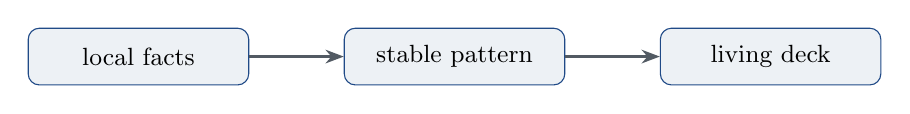
\begin{tikzpicture}[
  node distance=1.2cm,
  box/.style={draw=positive, rounded corners, fill=positive!8, minimum width=2.8cm, minimum height=0.72cm, font=\small},
  arr/.style={-{Stealth}, thick, draw=neutral}
]
  \node[box] (fact) {local facts};
  \node[box, right=of fact] (pattern) {stable pattern};
  \node[box, right=of pattern] (deck) {living deck};
  \draw[arr] (fact) -- (pattern);
  \draw[arr] (pattern) -- (deck);
\end{tikzpicture}
\end{center}
\end{frame}
\note{
这页是收束页。后续更新长期 deck 时，所有新增内容都应该回到这五条判断中：它是否改变项目主线？是否改变 benchmark 公平性？是否改变 symbolic/numeric 的解释？是否改变结果证据？是否改变平台差异解释？
}

\begin{frame}{References}
\small
\begin{thebibliography}{9}
\bibitem{petsc-dmplex}
PETSc Developers.
\newblock \emph{DMPlex: Unstructured Grids in PETSc}.
\newblock \url{https://petsc.org/main/manual/dmplex/}

\bibitem{petsc-section}
PETSc Developers.
\newblock \emph{DMPlexCreateSection manual page}.
\newblock \url{https://petsc.org/main/manualpages/DMPlex/DMPlexCreateSection/}

\bibitem{parallel-fem-assembly}
Comput. Methods Appl. Mech. Eng.
\newblock \emph{Parallel assembly of finite element matrices on multicore computers}.
\newblock \url{https://www.sciencedirect.com/science/article/pii/S0045782524003323}

\bibitem{sparse-atomic}
arXiv:2012.00585.
\newblock \emph{A flexible sparse matrix data format and parallel algorithms for assembly using atomic synchronisation primitives}.
\newblock \url{https://arxiv.org/abs/2012.00585}
\end{thebibliography}
\end{frame}
\note{
References slide 按 beamer skill 要求放在 Thank You 之前。这里只列长期 deck 中真正用于概念锚定的外部资料；项目事实仍以本地代码、docs 和 results 为准。
}

\begin{frame}{Thank You}
\begin{center}
{\Large Questions and project follow-up}

\vspace{1.0em}
\begin{tabular}{ll}
\toprule
复习入口 & \code{project\_long\_term\_beamer.tex} \\
来源索引 & \code{source\_index.md} \\
结果事实 & \code{results/} and benchmark reports \\
\bottomrule
\end{tabular}
\end{center}
\end{frame}
\note{
Thank You 不是结论页，真正的结论已经在“最后保留的主线判断”和 References 之前完成。这里作为 Q&A 入口。
}

\appendix

\begin{frame}{Backup Slides}
\begin{center}
{\Large Backup material for Q\&A}

\vspace{0.8em}
\begin{tabular}{ll}
\toprule
Backup & 用途 \\
\midrule
术语回查 & symbolic/numeric/scatter/closure \\
平台边界 & Intel taskset vs Apple QoS \\
维护检查 & source index 与 result figure paths \\
\bottomrule
\end{tabular}
\end{center}
\end{frame}

\begin{frame}{Backup: symbolic/numeric quick map}
\begin{center}
\begin{tabularx}{0.92\textwidth}{lXX}
\toprule
阶段 & 做什么 & 复用条件 \\
\midrule
symbolic & CSR pattern, element DOFs, scatter value indices & mesh topology 和 DOF numbering 不变 \\
numeric & compute $K_e$, add into CSR values & 每个 material/iteration/time-step 可重复 \\
direct no-symbolic & generate \code{(row,col,value)}, sort, reduce & 不复用 CSR/scatter path \\
\bottomrule
\end{tabularx}
\end{center}
\end{frame}

\begin{frame}{Backup: platform profile boundaries}
\begin{center}
\begin{tabularx}{0.94\textwidth}{lXX}
\toprule
平台 & profile 机制 & 汇报边界 \\
\midrule
Intel U7 265KF & Linux \code{taskset} affinity restriction & 可解释为 P/E-core resource restriction \\
Apple M4 Max & macOS QoS-biased scheduling & 不能写成 hard-pinned core affinity \\
cross-platform & schema records platform/profile fields & 趋势解释优先于绝对时间排名 \\
\bottomrule
\end{tabularx}
\end{center}
\end{frame}

\begin{frame}{Backup: maintenance verification commands}
\begin{center}
\begin{tabularx}{0.94\textwidth}{lX}
\toprule
检查项 & 命令 \\
\midrule
compile & \code{latexmk -xelatex -interaction=nonstopmode -halt-on-error project\_long\_term\_beamer.tex} \\
overlay ban & search for \code{\textbackslash pause}, \code{\textbackslash onslide}, \code{\textbackslash only}, and \code{\textbackslash uncover} \\
figure paths & extract every \code{\textbackslash resultfig\{...\}} path, then test that the referenced file exists \\
\bottomrule
\end{tabularx}
\end{center}
\end{frame}
\note{
这页用于未来维护时快速复查，不替代 README 中更完整的说明。
}

\end{document}
